\documentclass[paper=a4, fontsize=10pt]{jlreq}

\usepackage{amsmath, amssymb}
\usepackage{enumerate}
\usepackage{tikz}
\usepackage{listings, xcolor}
\usepackage{float}
\usepackage{graphicx}

\lstset{
  basicstyle = {\ttfamily},
  frame = {tbrl},
  breaklines = true,
  numbers = left,
  showspaces = false,
  showstringspaces = false,
  showtabs = false,
  keywordstyle = \color{blue},
  commentstyle = {\color[HTML]{1AB91A}},
  identifierstyle = \color{black},
  stringstyle = \color{brown},
  captionpos = t
}

\title{情報学群実験第3 最終レポート}
\author{学籍番号 1280391 \\ 細川 夏風}
\date{\today}

\begin{document}

\maketitle
\section{背景と目的}
近年，情報通信分野が発展している．中でも多くのデバイスがインターネットに接続されている．ネットワーク(以下:\texttt{NW})は現在の情報通信分野の基盤を支えている．これから先，多くのエンジニアが\texttt{NW}の設計に携わるか，それに近い業務を行うことになると予想される．そして，設計には\texttt{NW}の理解が必要である．しかし，\texttt{NW}について深く理解することは非常に難解なことである．そのため，今回は\texttt{Network Simulator2}(以下:\texttt{NS2})というソフトを用いて実際の\texttt{NW}の動作，主に\texttt{TCP/IP}というネットワークアーキテクチャのトランスポート層プロトコルの動作とパケットの挙動ついて考察と議論を行う．

\section{実験方法}
今回，私は\texttt{GID}，\texttt{SID}はともに$1$である．また，パケット損失率，スループットは以下の定義から算出される\cite{packet_chap}．
\begin{align*}
  T := \text{スループット}, D :&= \text{送信データ量}, t := \text{時間} \\
  T &= \frac{D}{t}
\end{align*}

\begin{align*}
  W := \text{ウィンドウサイズ}&, RTT := \text{往復遅延時間} \\
  T &= \frac{W}{RTT}
\end{align*}

\begin{align*}
  L := \text{パケット損失率}, N_{drop} := &\text{ドロップしたパケット数}, N_{sent} := \text{送信したパケット数} \\
  L = &\frac{N_{drop}}{N_{sent}} \times 100
\end{align*}

また，今回用いるソフトウェアとそのバージョンは以下のとおりである．

\vspace{2em}

\textbf{\texttt{Gnuplot}}
\begin{lstlisting}
  $ gnuplot --version
  gnuplot 6.0 patchlevel 0
\end{lstlisting}

\vspace{2em}

\textbf{\texttt{Network Sinulator2}}
\begin{lstlisting}
  $ ns
  % puts [ns-version]
  2.35
\end{lstlisting}

\subsection*{問題1}

ボトルネックリンクの帯域幅 \texttt{BW} を $1\ \mathrm{Mbps}$ から $10\ \mathrm{Mbps}$ まで変化させ，スループットおよびパケット損失率を測定した．

また，パケット損失率が $1.1\%$ を初めて超える帯域幅を \texttt{Efficiency Threshold} とした．

\begin{figure}[htbp]
\centering
\begin{tikzpicture}[>=latex]

\node[draw,circle] (n0) at (0,2) {$n_0$};
\node[draw,circle] (n1) at (0,-2) {$n_1$};

\node[draw,circle] (n2) at (4,0) {$n_2$};
\node[draw,circle] (n3) at (8,0) {$n_3$};

\node[draw,circle] (n4) at (12,2) {$n_4$};
\node[draw,circle] (n5) at (12,-2) {$n_5$};

% 左上
\draw (n0) -- (n2);
\node at (2,2.8) {$40\ \mathrm{Mbps}$};
\node at (2,1.6) {$6\ \mathrm{ms}$};

% 左下
\draw (n1) -- (n2);
\node at (2,-2.8) {$40\ \mathrm{Mbps}$};
\node at (2,-1.6) {$6\ \mathrm{ms}$};

% ボトルネック
\draw[very thick] (n2) -- (n3);
\node at (6,0.7) {\texttt{BW}};

% 右上
\draw (n3) -- (n4);
\node at (10,2.8) {$40\ \mathrm{Mbps}$};
\node at (10,1.6) {$6\ \mathrm{ms}$};

% 右下
\draw (n3) -- (n5);
\node at (10,-2.8) {$40\ \mathrm{Mbps}$};
\node at (10,-1.6) {$6\ \mathrm{ms}$};

\node at (-1.5,2) {\texttt{UDP}};
\node at (-2.0,-2) {\texttt{TCP}};

\node at (14.0,2) {\texttt{Null}};
\node at (14.0,-2) {\texttt{Sink}};

\end{tikzpicture}
\caption{問題1のネットワーク構成}
\end{figure}

\newpage

\subsection*{問題2}

ルータのバッファサイズ \texttt{B} を $1\ \mathrm{kbytes}$ から $10\ \mathrm{kbytes}$ まで変化させ，パケット損失率およびキューイング遅延を測定した．

さらに，バッファサイズ増加時におけるパケット損失率の変化について解析を行った．

\begin{figure}[htbp]
\centering
\begin{tikzpicture}[>=latex]

\node[draw,circle] (n0) at (0,2) {$n_0$};
\node[draw,circle] (n1) at (0,-2) {$n_1$};

\node[draw,circle] (n2) at (4,0) {$n_2$};
\node[draw,circle] (n3) at (8,0) {$n_3$};

\node[draw,circle] (n4) at (12,2) {$n_4$};
\node[draw,circle] (n5) at (12,-2) {$n_5$};

% 左上
\draw (n0) -- (n2);
\node at (2,2.8) {$40\ \mathrm{Mbps}$};
\node at (2,1.6) {$6\ \mathrm{ms}$};

% 左下
\draw (n1) -- (n2);
\node at (2,-2.8) {$40\ \mathrm{Mbps}$};
\node at (2,-1.6) {$6\ \mathrm{ms}$};

% ボトルネック
\draw[very thick] (n2) -- (n3);
\node at (6,0.7) {\texttt{BW}$=3$\texttt{Mdps}};
\node at (6, -0.7) {$20ms$};


% 右上
\draw (n3) -- (n4);
\node at (10,2.8) {$40\ \mathrm{Mbps}$};
\node at (10,1.6) {$6\ \mathrm{ms}$};

% 右下
\draw (n3) -- (n5);
\node at (10,-2.8) {$40\ \mathrm{Mbps}$};
\node at (10,-1.6) {$6\ \mathrm{ms}$};

\node at (-1.5,2) {\texttt{UDP}};
\node at (-2.0,-2) {\texttt{TCP}};

\node at (14.0,2) {\texttt{Null}};
\node at (14.0,-2) {\texttt{Sink}};

\end{tikzpicture}
\caption{問題2のネットワーク構成}
\end{figure}

\subsection*{問題3}

\texttt{TCP Tahoe} を用いて通信を行い，\texttt{cwnd} および \texttt{ssthresh} の時間変化を観測した．

また，最大ウィンドウサイズおよび送信スループットを算出した．

\begin{figure}[htbp]
\centering
\begin{tikzpicture}[>=latex]

\node[draw,circle] (n0) at (0,2) {$n_0$};
\node[draw,circle] (n1) at (0,-2) {$n_1$};

\node[draw,circle] (n2) at (4,0) {$n_2$};
\node[draw,circle] (n3) at (8,0) {$n_3$};

\node[draw,circle] (n4) at (12,2) {$n_4$};
\node[draw,circle] (n5) at (12,-2) {$n_5$};

% 左上
\draw (n0) -- (n2);
\node at (2,2.8) {$25\ \mathrm{Mbps}$};
\node at (2,1.6) {$5\ \mathrm{ms}$};

% 左下
\draw (n1) -- (n2);
\node at (2,-2.8) {$25\ \mathrm{Mbps}$};
\node at (2,-1.6) {$5\ \mathrm{ms}$};

% ボトルネック
\draw[very thick] (n2) -- (n3);
\node at (6,0.7) {\texttt{BW}$=2$};
\node at (6, -0.7) {\texttt{B}};

% 右上
\draw (n3) -- (n4);
\node at (10,2.8) {$25\ \mathrm{Mbps}$};
\node at (10,1.6) {$5\ \mathrm{ms}$};

% 右下
\draw (n3) -- (n5);
\node at (10,-2.8) {$25\ \mathrm{Mbps}$};
\node at (10,-1.6) {$5\ \mathrm{ms}$};

\node at (-2.0,2) {\texttt{TCP}};
\node at (-2.0,-2) {\texttt{TCP}};

\node at (14.0,2) {\texttt{Sink}};
\node at (14.0,-2) {\texttt{Sink}};

\end{tikzpicture}
\caption{問題3のネットワーク構成}
\end{figure}

\subsection*{問題4}

\texttt{TCP Reno} を用いて通信を行い，\texttt{cwnd} および \texttt{ssthresh} の変化を \texttt{TCP Tahoe} と比較した．

また，輻輳によるパケット損失数およびシーケンス番号を確認した．

\begin{figure}[htbp]
\centering
\begin{tikzpicture}[>=latex]

\node[draw,circle] (n0) at (0,2) {$n_0$};
\node[draw,circle] (n1) at (0,-2) {$n_1$};

\node[draw,circle] (n2) at (4,0) {$n_2$};
\node[draw,circle] (n3) at (8,0) {$n_3$};

\node[draw,circle] (n4) at (12,2) {$n_4$};
\node[draw,circle] (n5) at (12,-2) {$n_5$};

% 左上
\draw (n0) -- (n2);
\node at (2,2.8) {$25\ \mathrm{Mbps}$};
\node at (2,1.6) {$5\ \mathrm{ms}$};

% 左下
\draw (n1) -- (n2);
\node at (2,-2.8) {$25\ \mathrm{Mbps}$};
\node at (2,-1.6) {$5\ \mathrm{ms}$};

% ボトルネック
\draw[very thick] (n2) -- (n3);
\node at (6,0.7) {\texttt{BW}$=2$};
\node at (6, -0.7) {\texttt{B}};

% 右上
\draw (n3) -- (n4);
\node at (10,2.8) {$25\ \mathrm{Mbps}$};
\node at (10,1.6) {$5\ \mathrm{ms}$};

% 右下
\draw (n3) -- (n5);
\node at (10,-2.8) {$25\ \mathrm{Mbps}$};
\node at (10,-1.6) {$5\ \mathrm{ms}$};

\node at (-2.0,2) {\texttt{TCP}};
\node at (-2.0,-2) {\texttt{TCP}};

\node at (14.0,2) {\texttt{Sink}};
\node at (14.0,-2) {\texttt{Sink}};

\end{tikzpicture}
\caption{問題4のネットワーク構成}
\end{figure}

\section{結果}

\subsection*{問題1-1}

図\ref{fig:throughput}にスループットと帯域幅の関係を、図\ref{fig:droprate}にパケット損失率と帯域幅の関係を示す。

\begin{figure}[htbp]
    \centering
    % 画像の幅をテキスト幅の80%に設定
    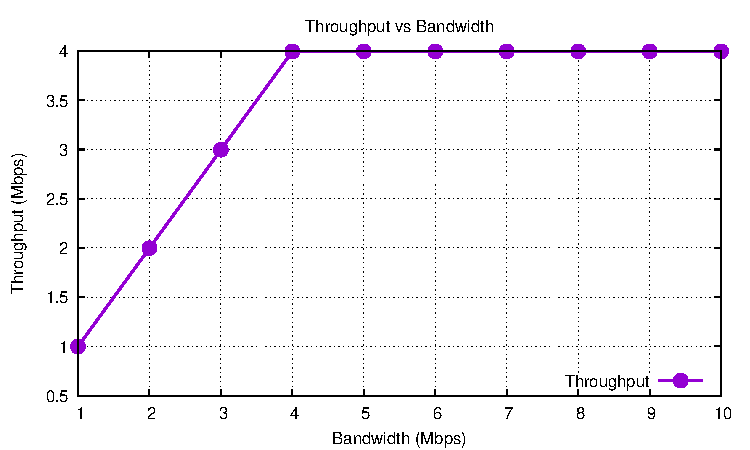
\includegraphics[width=0.8\linewidth]{kadai1_throughput.pdf}
    \caption{スループットと帯域幅の関係}
    \label{fig:throughput}
\end{figure}

\begin{figure}[htbp]
    \centering
    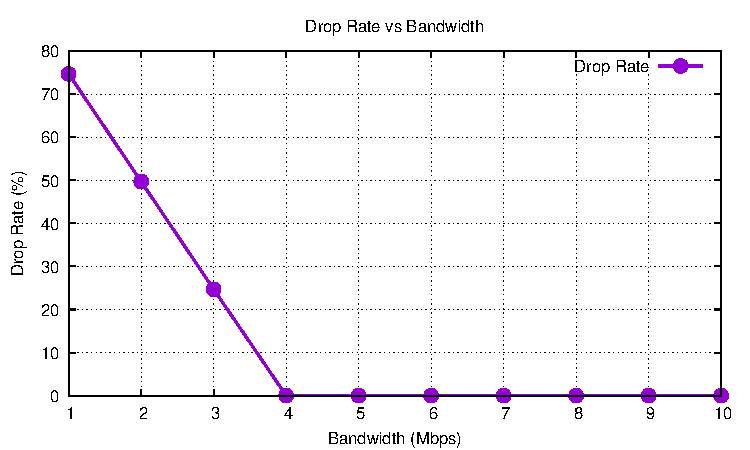
\includegraphics[width=0.8\linewidth]{kadai1_droprate.pdf}
    \caption{パケット損失率と帯域幅の関係}
    \label{fig:droprate}
\end{figure}

\subsection*{問題1-2}

付録\ref{src:kadai1-1.sh}から得られる値は次にようになる．

\begin{table}[htbp]
  \centering
  \caption{帯域幅に対するスループットおよびパケット損失率の測定結果}
  \label{tab:kadai1_result}
  \begin{tabular}{ccc}
    \hline
    帯域幅 (Mbps) & スループット (Mbps) & パケット損失率 (\%) \\
    \hline
    1  & 0.998800 & 74.682405 \\
    2  & 1.997999 & 49.694908 \\
    3  & 2.996999 & 24.687406 \\
    4  & 3.995998 &  0.000000 \\
    5  & 3.996079 &  0.000000 \\
    6  & 3.996132 &  0.000000 \\
    7  & 3.996170 &  0.000000 \\
    8  & 3.996199 &  0.000000 \\
    9  & 3.996221 &  0.000000 \\
    10 & 3.996239 &  0.000000 \\
    \hline
  \end{tabular}
\end{table}

以上の結果から，\texttt{BW}が$3$\texttt{Mbps}のときに\texttt{Efficiency Threshold}を下回っている事がわかる．よって，\texttt{Efficiency Threshold}は$3$\texttt{Mbps}である．

\subsection*{問題1-3}

\label{kadai1-3}

上記のデータ群から一定値を超えるとスループットが一定値で飽和していることがわかる．これは，送信データ量より帯域幅が大きくなったためである．$1$秒間に送信可能なデータ量が実際に送信しているデータ量よりも大きい場合，パケットが送信中にバッファから溢れてドロップすることがなくなるのだ．よって，パケット損失率も$0\%$であり，スループットが一定値で飽和している事がわかる．

\subsection*{問題2-1}

図\ref{fig:kadai2_droprate}にバッファサイズとパケット損失率の関係を示す．

\begin{figure}[htbp]
  \centering
  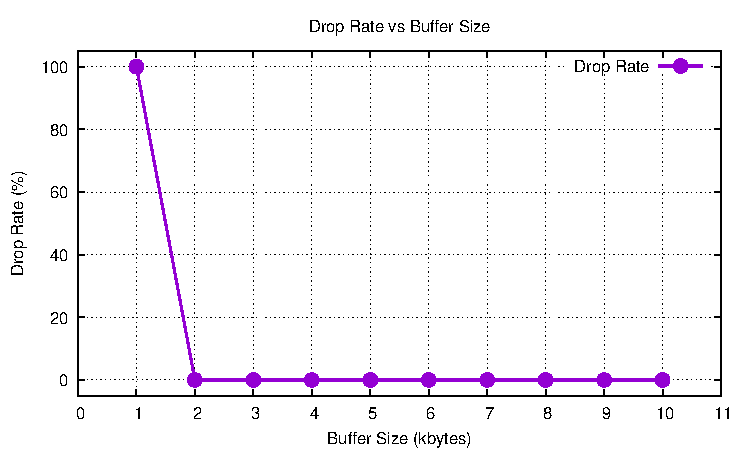
\includegraphics[width=0.8\linewidth]{kadai2_droprate.pdf}
  \caption{バッファサイズとパケット損失率}
  \label{fig:kadai2_droprate}
\end{figure}

\subsection*{問題2-2}

付録\ref{src:kadai2-2.sh}から，その結果は$0$であった．よって，最大バッファサイズにおけるキューイング遅延は無いと言える．また，これはデータからも考えられる．表\ref{tab:kadai1_result}でも最大バッファサイズのパケット損失率は$0\%$であり，送信データ量に対して帯域幅が大きいため起こっているからであると考えられる．そのため，バッファに格納される時間が著しく短いか，ほとんど無いと言える．

\newpage

\subsection*{問題2-3}

バッファサイズとパケット損失率の関係を以下のグラフに示す．このデータは意図的に帯域幅を小さく設定し，パケット損失率が大きくなるように設定している．

\begin{figure}[htbp]
  \centering
  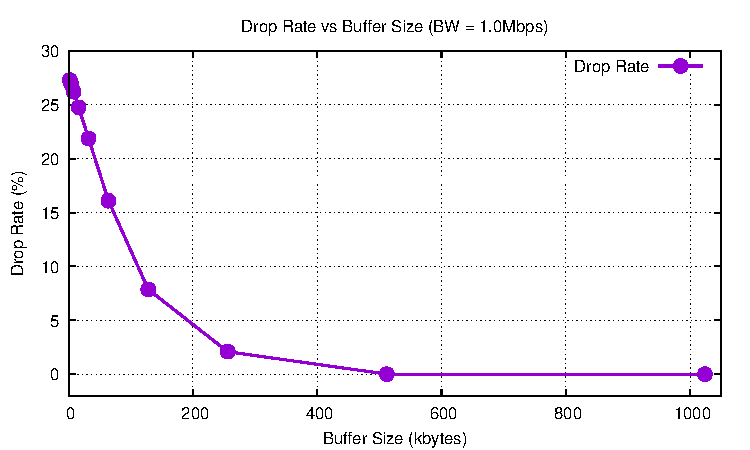
\includegraphics[width=0.8\linewidth]{kadai2_nonlinear.pdf}
  \caption{バッファサイズとパケット損失率}
  \label{fig:kadai2_nonlinear}
\end{figure}

\subsection*{問題3-1}

\texttt{cwnd}(送信ウィンドウサイズ)，\texttt{ssthresh}(スロースタート閾値)の時間変化を以下のグラフに示す．

\begin{figure}[htbp]
  \centering
  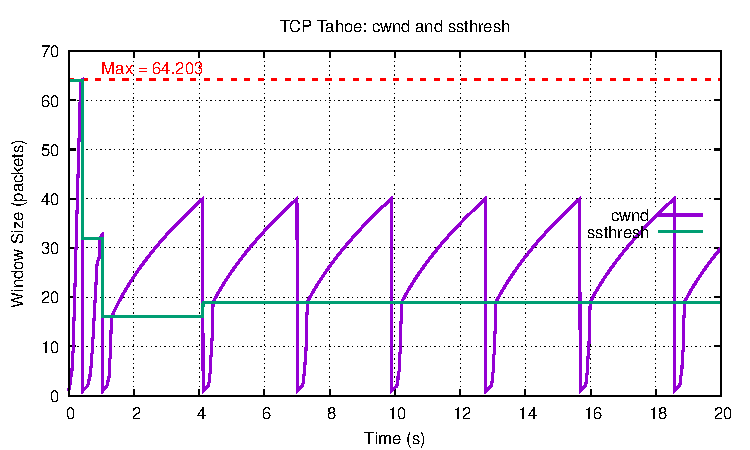
\includegraphics[width=0.8\linewidth]{kadai3_tahoe.pdf}
  \caption{cwndとssthreshの時間変化におけるグラフ}
  \label{fig:kadai3_tahoe}
\end{figure}

\subsection*{問題3-2}

付録\ref{src:kadai3-2.sh}の結果から値は$0.029091$であった．よって，$11$\texttt{ms}のまでスループットは$0.029091$\texttt{Mbps}である．

\subsection*{問題3-3}

図\ref{fig:kadai3_tahoe}から，\texttt{ssthresh}は一度減少したあとわずかに上昇したように見える．

\subsection*{問題4-1}

\texttt{cwnd}(送信ウィンドウサイズ)，\texttt{ssthresh}(スロースタート閾値)の時間変化を以下のグラフに示す．

\begin{figure}[htbp]
  \centering
  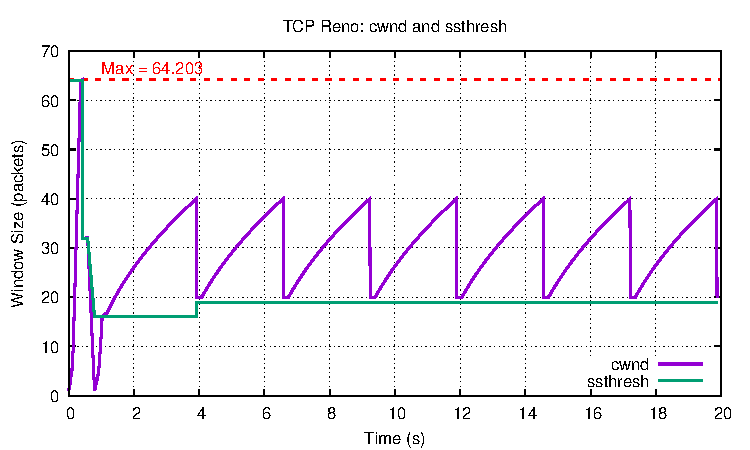
\includegraphics[width=0.8\linewidth]{kadai4_reno.pdf}
  \caption{cwndとssthreshの時間変化におけるグラフ}
  \label{fig:kadai4_reno}
\end{figure}

\subsection*{問題4-2}

付録\ref{src:kadai4-2.sh}の結果から，出力された値は$0.029091$である．よって$11$\texttt{ms}までのスループットは$0.029091$\texttt{Mbps}である．

\subsection*{問題4-3}

\label{kadai4-3}

付録\ref{src:kadai4-3.sh}の結果から，出力された値の集合は\\ 
$L = \{ 76, 78, 80, 82, 84, 86, 88, 90, 92, 94, 96, 98, 100, 102, 104, 106, 108, 110, 112, 114, 116, 118, 120, 122, 124, 126, \\ 801, 1440, 2079, 2718, 3357, 3996, 4635 \} $ \\
である．これはプログラムからドロップしたシーケンス番号の集合である．この集合の濃度$|L|$は$33$である．

\section{考察}

\subsection*{問題1}

この問ではボトルネックリンクにおける帯域幅がパケットの損失率とスループットに与える影響を示している．図\ref{fig:throughput}，\ref{fig:droprate}，表\ref{tab:kadai1_result}から帯域幅の上昇はパケットの損失率を減少させ，スループットを上昇させる効果があることがわかる．その上昇量はパケット損失率は割合のためもちろん$0\%$で停止する．それに加えて，スループットもある帯域幅から極端に上昇量が小さくなるか$0$になる場合がある．これは\ref{kadai1-3}節にもあるが，送信しているデータ量に比べて帯域幅が大きくなったためであると考えられる．

\subsection*{問題2}

この問ではバッファサイズがパケット損失率，遅延に与える影響を示している．図\ref{fig:kadai2_droprate}，\ref{fig:kadai2_nonlinear}より，バッファサイズを上昇させることによってパケット損失率が小さくなるか，$0\%$になっていることがわかる．これはホップのバッファ内に格納できるパケットの量が多くなっているため，溢れてドロップするという事が少なくなるためであると考えられる．最大バッファサイズにおける遅延はほとんど無いという結果になった．しかし，これは帯域幅がもっと小さくかつバッファサイズが十分に大きい場合，バッファ内に格納される時間が大きいため遅延時間が長くなるというケースが考えられる．

\subsection*{問題3}

\label{kadai3}

この問では\texttt{tahoe}における\texttt{cwnd}と\texttt{ssthresh}の時間における推移を示している．図\ref{fig:kadai3_tahoe}から\texttt{ssthresh}は一度減少した後，わずかに上昇している．これは最適化の結果である．\texttt{tahoe}では，輻輳を検知すると\texttt{ssthresh}の$\frac{1}{2}$倍し，\texttt{cwnd}を$1$にして通信を再開する．この\texttt{ssthresh}が上昇すると指数的に上昇する時間がわずかに増加するため，その分パケットが多く送られることになる．よって，単位時間あたりの送信されるパケットが増加すると考えられる．

\subsection*{問題4}

この問では\texttt{reno}における\texttt{cwnd}と\texttt{ssthresh}の時間における推移を表してる．図\ref{fig:kadai4_reno}から\texttt{ssthresh}は一度に減少したあと，上昇している．この方式でも\ref{kadai3}節と同じことが言える．つまり，最適化の結果であると考えられる．しかし，\texttt{reno}は輻輳を検知すると\texttt{cwnd}を$\frac{1}{2}$倍して通信を再開する．これはあくまでパケットの受信順番の入れ違いで発生してしまった輻輳だと検知し，大きく\texttt{cwnd}を落とさずに高速な通信を維持する方法である\cite{rfc5681}．しかし，\ref{kadai4-3}節から，合計$33$回はドロップが発生していることがわかる．高速に通信を行おうとすれば必然的にドロップ回数は多くなってしまうという事がわかる．これは通信の帯域幅の限界に近い部分まで通信を行うというアルゴリズムが作動しているからとも言える．

\begin{thebibliography}{99}
  \bibitem{packet_chap} パケットキャプチャ実践技術 \texttt{Wireshark}によるパケット解析 実践編, 竹下恵, 株式会社リックテレコム, 2012年12月5日
  \bibitem{rfc5681}
M. Allman, V. Paxson, and E. Blanton,
``{TCP} Congestion Control,''
RFC 5681, Sep. 2009.
[Online]. Available: \texttt{https://www.rfc-editor.org/rfc/rfc5681}
\end{thebibliography}


\section{作成したシェルスクリプト}
問題1の自動実行とデータ抽出のために作成したシェルスクリプト (\texttt{kadai1-1.sh}) を以下に示す。

% language=bashを指定することで、シェルスクリプト用の色分けが行われます
\lstinputlisting[language=bash, caption={問題1の実行スクリプト (kadai1-1.sh)}, label={src:kadai1-1.sh}]{kadai1-1.sh}

\lstinputlisting[language=bash, caption={問題2-1の実行スクリプト (kadai2-1.sh)}, label={src:kadai2-1.sh}]{kadai2-1.sh}

\lstinputlisting[language=bash, caption={問題2-2の実行スクリプト (kadai2-2.sh)}, label={src:kadai2-2.sh}]{kadai2-2.sh}

\lstinputlisting[language=bash, caption={問題2-3の実行スクリプト (kadai2-3.sh)}, label={src:kadai2-3.sh}]{kadai2-3.sh}

\lstinputlisting[language=bash, caption={問題3-2の実行スクリプト (kadai3-2.sh)}, label={src:kadai3-2.sh}]{kadai3-2.sh}

\lstinputlisting[language=bash, caption={問題4-2の実行スクリプト (kadai4-2.sh)}, label={src:kadai4-2.sh}]{kadai4-2.sh}

\lstinputlisting[language=bash, caption={問題4-3の実行スクリプト (kadai4-3.sh)}, label={src:kadai4-3.sh}]{kadai4-3.sh}
\end{document}
